\documentclass[12pt,a4paper]{article}
\usepackage[top=25.4mm, bottom=25.4mm, left=19.1mm, right=19.1mm]{geometry}

\usepackage[latin2]{inputenc}
\usepackage{graphicx}
\graphicspath{ {./images/} }
\usepackage{ulem}
\usepackage{amsmath}
\usepackage[document]{ragged2e}

\setlength{\parindent}{4em}
\setlength{\parskip}{1em}
\usepackage{hyperref}

\usepackage{fancyhdr}
\pagestyle{fancy}
\fancyhf{}
\fancyhead[LO]{\textbf{\small IoT and Smart Analytics}\\
\text{\small A Program by IIITH and TalentSprint}}

\usepackage{xcolor}
\usepackage{lipsum}

\rhead{\begin{picture}(0,0) \put(-250,-2){
\includegraphics[width=9cm]{EXP_08_Images/ts-iisc-logo-pr.png}} \end{picture}}
\cfoot{\thepage}


\begin{document}

\begin{center}

\textbf{\large \\EXPERIMENT 20 }\\[6pt]
\text{ESP32-ESP32 Two-way Communication}
\end{center}

\textbf{\large LEARNING OBJECTIVES:}\\[3pt]
At the end of this experiment, participants will be able to:\vspace{-6mm}
\begin{enumerate}
\setlength\itemsep{-0.3em}
\item Understand how to communicate between two ESP32 using ESP-now
\end{enumerate}

\textbf{\large APPARATUS REQUIRED:}\\
\vspace{-3mm}
\begin{enumerate}
 \setlength\itemsep{-0.3em}
\item ESP32 Module -2pcs
\item Micro USB cable - 2pcs
\item Arduino IDE
\end{enumerate}

\begin{justify}
\textbf{\large THEORY}\\[3pt]
\textbf{Introduction :} ESP-NOW is a connectionless Wi-Fi communication protocol that Espressif defines. In ESP-NOW, the data is encapsulated in the vendor-specific action frame and then transmitted from one Wi-Fi device to another without connection. ESP-NOW is widely used in intelligent light, remote controlling, sensors, etc. It features short packet transmission.\par
\noindent More details about the protocol working can be found in this \href{https://docs.espressif.com/projects/esp-idf/en/latest/esp32/api-reference/network/esp_now.html}{link}. The pairing between devices is needed before their communication. After finishing the pairing, the connection is safe and peer-to-peer, requiring no handshake. It means that after pairing the device with each other, the connection is persistent. If suddenly one of the boards loses power or resets, when it restarts, it automatically connects to its peer to continue communication. ESP-NOW is a fast communication protocol which can be used to exchange small messages which are up to 250 bytes between ESP32 boards.\par
\noindent ESP-NOW is a very versatile protocol, and we can have one-way or two-way communication in different setups.


\begin{center} 
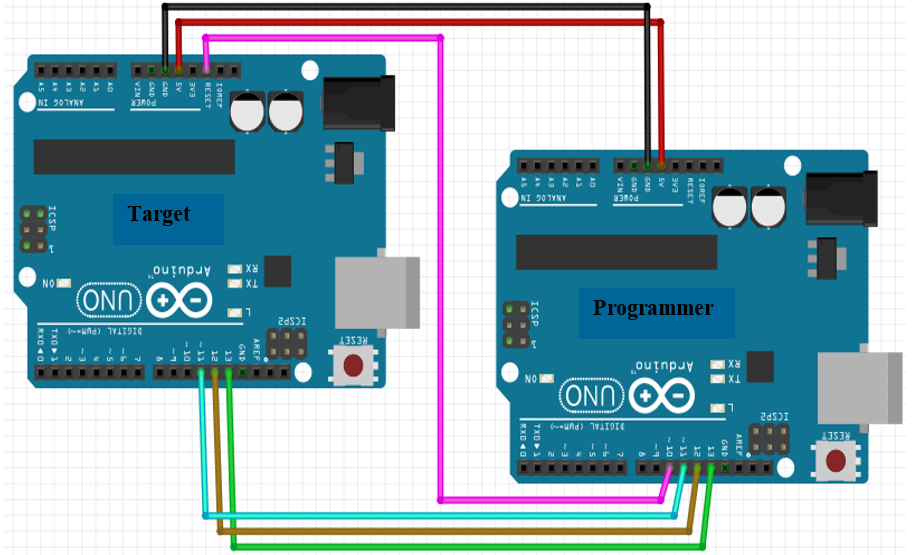
\includegraphics[scale=0.6]{EXP_20_Images/fig1.png}
\end{center}
\begin{center} {Figure 1. Possible connections using ESP-NOW}\end{center}

\textbf{Overview :}
\vspace{-3mm}
\begin{itemize}
\setlength\itemsep{-0.3em}
\item In this experiment, we'll have two ESP32 boards. 
\item  One board generates a random number and sends it to the other board via ESP-NOW;
\item  The other board adds, or any other decided operation with a number decided earlier and sent back to the previous board;
\item  When the first board receives the readings, it displays them on the serial monitor;
\item  Each board needs to know the other board's MAC address to send the message.
\end{itemize}
\end{justify}


\textbf{\large Code :}\\[6pt]
Firstly we need to obtain the Mac addresses of both boards. Use the following code to get the Mac address for both boards.

\#include $<WiFi.h>$\\
void setup()\\
\{\\
  Serial.begin(115200);\\
  WiFi.mode(WIFI\_STA);\\
  Serial.println(WiFi.macAddress());\\
\}\\
void loop()\{ \}\\[15pt]


\underline{Expected output:}\\
The serial monitor prints the Wi-Fi Mac address of the ESP32 board. \\
In this case, the mac addresses are :\\
Board1 : 08:3A:F2:50:E1:00\\
Board2 : 08:3A:F2:52:21:68\\
Next, the boards need to be configured to communicate two-way with the given mac addresses.\\
\textbf{Note:}\\
Open two different instances of Arduino to be able to open two serial ports using two serial monitors.\\
Upload the respective codes on the boards and observe the values on two different serial monitors.

\textbf{\large Code For board-1 :}\\[6pt]

\#include $<esp\_now.h>$\\
\#include $<WiFi.h>$\\

\textcolor{blue}{// REPLACE IT WITH THE MAC Address of your receiver 
:\\08:3A:F2:52:21:68}\\
uint8\_t broadcastAddress[ ] = \{0x08, 0x3A, 0xF2, 0x52, 0x21, 0x68\};\\
int incoming\_val;\\
\textcolor{blue}{// Variable to store if sending of the data was successful}\\
String success;\\
\textcolor{blue}{//Structure example to send data}\\
\textcolor{blue}{//Must match the receiver structure}\\
typedef struct struct\_message \{float val;\}\\
struct\_message;\\
\textcolor{blue}{// Create a struct\_message called sensor\_data }\\
struct\_message sensor\_data;\\

\textcolor{blue}{// Create a struct\_message to hold incoming data}\\
struct\_message incoming\_data;\\

\textcolor{blue}{// Callback when data has been sent}\\
void OnDataSent(const uint8\_t *mac\_addr, esp\_now\_send\_status\_t status)\\
\{\\
\textcolor{blue}{// print the last packet status}\\
  Serial.print("\textbackslash r\textbackslash nLast Packet Status:\t");\\
  Serial.println(status $== $ESP\_NOW\_SEND\_SUCCESS ?\\ "Delivery Success" : "Delivery Fail");\\ 
  \textcolor{blue}{//checking for the esp\_now status}\\
  if (status ==0)\\
  \{ success = "Delivery Success :)";\}\\
  else \{ success = "Delivery Fail :("; \}\\
\}\\

\textcolor{blue}{// Function Callback when the data has been obtained}\\
void OnDataRecv(const uint8\_t * mac, const uint8\_t *incomingData, int len)\\
\{\\

  memcpy(\&incoming\_data, incomingData, sizeof(incoming\_data));\\
  Serial.print("Bytes received: ");\\
  Serial.println(len);\\
  incoming\_val = incoming\_data.val;\\
\}\\[15pt]
 
void setup()\\
\{
  \textcolor{blue}{// Init Serial Monitor}\\
  Serial.begin(115200);

  \textcolor{blue}{// Set device as a Wi-Fi Station}\\
  WiFi.mode(WIFI\_STA);\\

  \textcolor{blue}{// Init ESP-NOW}\\
  if (esp\_now\_init() != ESP\_OK)\\
  \{\\
    Serial.println("Error initializing ESP-NOW");\\
    return;\\
  \}\\
  \textcolor{blue}{// Once ESPNow is successfully Initialised, we will register for Send CB to get the status of Trasnmitted packet}\\
  esp\_now\_register\_send\_cb(OnDataSent);\\
  \textcolor{blue}{// Register peer}\\
  esp\_now\_peer\_info\_t peerInfo;\\
  memcpy(peerInfo.peer\_addr, broadcastAddress, 6);\\
  peerInfo.channel = 0; \\
  peerInfo.encrypt = false;\\
  \textcolor{blue}{// Add peer}\\      
  if (esp\_now\_add\_peer(\&peerInfo) != ESP\_OK)\\
  \{\\ 
    Serial.println("Failed to add peer");\\
    \textcolor{blue}{//check for peer connection}\\
    return;\\
  \}\\
  \textcolor{blue}{// Registering for a callback function that will be called when \\// the data is received}\\
  esp\_now\_register\_recv\_cb(OnDataRecv);\\
\}\\[15pt]
 
void loop() \\
\{\\  
sensor\_data.val=random(30);\\
  Serial.print("Value sent:");\\
  Serial.println(sensor\_data.val);\\
 \textcolor{blue}{ // Send message via ESP-NOW}\\
  esp\_err\_t result = esp\_now\_send(broadcastAddress, (uint8\_t *) \&sensor\_data, sizeof(sensor\_data));\\
   
  if (result == ESP\_OK) \\
  \{\\
    Serial.println("Sent with success");\\
  \}\\
  else \{ Serial.println("Error sending the data");\}\\
  delay(10000);\\
  Serial.println("INCOMING READINGS");\\
  Serial.print("Changed value: ");\\
  Serial.println(incoming\_data.val);\\
  Serial.println(" \%\%\%\%\%\%\%\%\%\%\%\%\%\%\% ");\\
\}


\vspace{5mm}
\textbf{\large Code For board-2 :}\\[6pt]

\#include $<esp\_now.h>$\\
\#include $<WiFi.h>$\\

\textcolor{blue}{// REPLACE IT WITH THE MAC Address of your receiver 
:\\08:3A:F2:50:E1:00}\\
uint8\_t broadcastAddress[ ] = \{0x08, 0x3A, 0xF2, 0x50, 0xE1, 0x00\};\\
int incoming\_val;\\
\textcolor{blue}{// Variable to store if sending of the data was successful}\\
String success;\\
\textcolor{blue}{//Structure example to send data}\\
\textcolor{blue}{//Must match the receiver structure}\\
typedef struct struct\_message \{float val;\}\\
struct\_message;\\
\textcolor{blue}{// Create a struct\_message called sensor\_data }\\
struct\_message sensor\_data;\\

\textcolor{blue}{// Create a struct\_message to hold incoming data}\\
struct\_message incoming\_data;\\

\textcolor{blue}{// Callback when data has been sent}\\
void OnDataSent(const uint8\_t *mac\_addr, esp\_now\_send\_status\_t status)\\
\{\\
\textcolor{blue}{// print the status of  last send packet }\\
  Serial.print("\textbackslash r\textbackslash nLast Packet Status:\t");\\
  Serial.println(status $== $ESP\_NOW\_SEND\_SUCCESS ?\\ "Delivery Success" : "Delivery Fail");\\ 
  \textcolor{blue}{//checking for the esp\_now status}\\
  if (status ==0)\\
  \{ success = "Delivery Success :)";\}\\
  else \{ success = "Delivery Fail :("; \}\\
\}\\

\textcolor{blue}{// Function Callback when the data has been received}\\
void OnDataRecv(const uint8\_t * mac, const uint8\_t *incomingData, int len)\\
\{\\

  memcpy(\&incoming\_data, incomingData, sizeof(incoming\_data));\\
  Serial.print("Bytes received: ");\\
  Serial.println(len);\\
  incoming\_val = incoming\_data.val;\\
\}\\[15pt]
 
void setup()\\
\{
  \textcolor{blue}{// Init Serial Monitor}\\
  Serial.begin(115200);

  \textcolor{blue}{// Set device as a Wi-Fi Station}\\
  WiFi.mode(WIFI\_STA);\\

  \textcolor{blue}{// Init ESP-NOW}\\
  if (esp\_now\_init() != ESP\_OK)\\
  \{\\
    Serial.println("Error initializing ESP-NOW");\\
    return;\\
  \}\\
  \textcolor{blue}{// Once ESPNow is successfully Initialised, we will register for Send CB to get the status of Trasnmitted packet}\\
  esp\_now\_register\_send\_cb(OnDataSent);\\
  \textcolor{blue}{// Register peer}\\
  esp\_now\_peer\_info\_t peerInfo;\\
  memcpy(peerInfo.peer\_addr, broadcastAddress, 6);\\
  peerInfo.channel = 0; \\
  peerInfo.encrypt = false;\\
  \textcolor{blue}{// Add peer}\\      
  if (esp\_now\_add\_peer(\&peerInfo) != ESP\_OK)\\
  \{\\ 
    Serial.println("Failed to add peer");\\
    \textcolor{blue}{//check for peer connection}\\
    return;\\
  \}\\
  \textcolor{blue}{// Registering for a callback function that will be called when \\// the data is received}\\
  esp\_now\_register\_recv\_cb(OnDataRecv);\\\textcolor{blue}{// Ondata callback}\\
\}\\[15pt]
 
void loop() \\
\{\\  
Serial.println("\%\%\%\%\%\%\%\%\%\%\%\%\%\%");\\
Serial.println("INCOMING READINGS");\\
  Serial.print("Value :");\\
  Serial.println(incoming\_data.val);\\
  sensor\_data.val=incoming\_data.val+2;\\
  Serial.print("Value being sent back:");\\
  Serial.println(sensor\_data.val);\\
 \textcolor{blue}{ // Send message via ESP-NOW}\\
  esp\_err\_t result = esp\_now\_send(broadcastAddress, (uint8\_t *) \&sensor\_data, sizeof(sensor\_data));\\
   
  if (result == ESP\_OK) \\
  \{\\
    Serial.println("Sent with success");\\
  \}\\
  else \{ Serial.println("Error sending the data");\}\\
  delay(10000);\\
\}











\setlength{\parindent}{0pt}
\begin{justify}
\begin{center} 
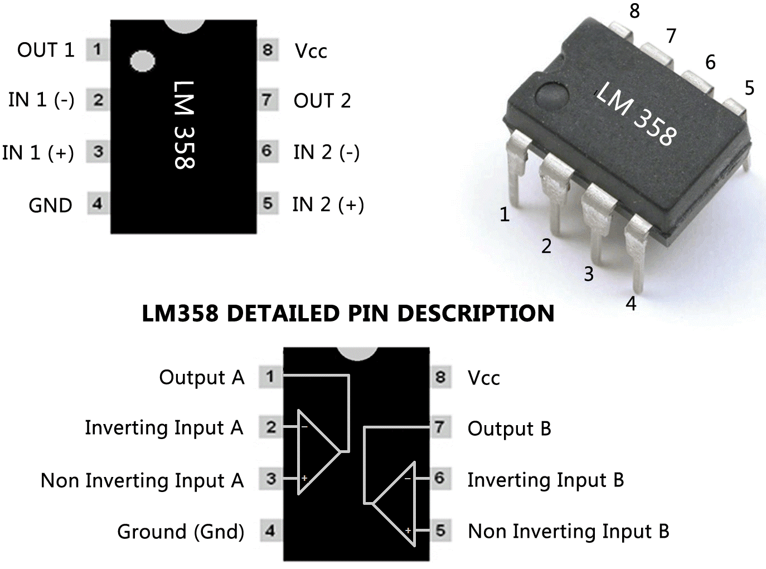
\includegraphics[scale=0.4]{EXP_20_Images/fig2.PNG}
\end{center}
\begin{center} {Figure 2.Board1 and Board2 Serial Monitor output}\end{center}\\

\textbf{\large REFERENCES:}
\vspace{-6mm}
\begin{enumerate}
\setlength\itemsep{-0.3em}
\item  \href {https://docs.espressif.com/projects/esp-idf/en/latest/esp32/api-reference/network/esp_now.html}{ESP-Now}
\item  \href {https://randomnerdtutorials.com/esp-now-two-way-communication-esp32/ }{ESP-Now Two Way Communication}
\end{enumerate}
\end{justify}
\end{document}